\documentclass{amsart}
%DIF LATEXDIFF DIFFERENCE FILE
%DIF DEL diff1.tex   Mon Aug 22 07:54:28 2022
%DIF ADD diff2.tex   Mon Aug 22 07:54:28 2022
\synctex=1

%=================================================================
% 
\newcount\DraftStatus  % 0 suppresses notes to selves in text
\DraftStatus=1   % TODO: set to 0 for final version
%=================================================================

%=================================================================
\usepackage{comment}
%=================================================================
%
\includecomment{JournalOnly}  
\includecomment{ConferenceOnly}  
\includecomment{TulipStyle}
%
%=================================================================
%=================================================================
% gitlatexdiff
%
%  https://gitlab.com/git-latexdiff/git-latexdiff
%=================================================================
%  git latexdiff HEAD  HEAD~5 --main templatex.tex
%  git latexdiff HEAD~1  --main templatex.tex
%  View pdf to see difference
%
%=================================================================
%
% Todo Notes for marginal comments
% 
%\newcount\DraftStatus  % 0 suppresses notes to selves in text
%\DraftStatus=1   % TODO: set to 0 for final version
\ifnum\DraftStatus=1
	\usepackage[draft,colorinlistoftodos,color=orange!30]{todonotes}
\else
	\usepackage[disable,colorinlistoftodos,color=blue!30]{todonotes}
\fi 
%\usepackage[disable]{todonotes} % notes not showed
%\usepackage[draft]{todonotes}   % notes showed
%
\makeatletter
 \providecommand\@dotsep{5}
 \def\listtodoname{List of Todos}
 \def\listoftodos{\@starttoc{tdo}\listtodoname}
 \makeatother
%
%=================================================================
%
\usepackage{color}
\newcommand{\draftnote}[3]{ 
	\todo[author=#2,color=#1!30,size=\footnotesize]{\textsf{#3}}	}
% TODO: add yourself here:
%
\newcommand{\gangli}[1]{\draftnote{blue}{GLi:}{#1}}
\newcommand{\qwu}[1]{\draftnote{red}{QWu:}{#1}}
\newcommand{\gliMarker}
	{\todo[author=GLi,size=\tiny,inline,color=blue!40]
	{Gang Li has worked up to here.}}
\newcommand{\qwuMarker}
	{\todo[author=QWu,size=\tiny,inline,color=red!40]
	{Qiong Wu has worked up to here.}}
%=================================================================

%=================================================================
%
% general packages
%  https://en.wikibooks.org/wiki/Category:Book:LaTeX
%  https://en.wikibooks.org/wiki/LaTeX/Package_Reference
%
%=================================================================
\usepackage{graphicx}
\graphicspath{{./figures/}{./graphics/}{./graphics/logos/}}

\usepackage{algorithm}
\usepackage{algorithmic}
\usepackage{breqn}
\usepackage{subcaption}
\usepackage{multirow}
\usepackage{psfrag}
\usepackage{url}
\usepackage[colorlinks,citecolor=blue]{hyperref}
%\usepackage{hyperref}
%\usepackage[colorlinks]{hyperref}
%\usepackage{cite}
\usepackage{cleveref}
\usepackage{booktabs}
\usepackage{rotating}
\usepackage{colortbl}
\usepackage{paralist}
%\usepackage{geometry}
\usepackage{epstopdf}
\usepackage{nag}
\usepackage{microtype}
\usepackage{siunitx}
\usepackage{nicefrac}
%\usepackage{breakurl}
\usepackage{fontawesome}
\usepackage{xcolor}
\usepackage{multicol}
\usepackage{wrapfig}
\usepackage{todonotes}
\usepackage{tablefootnote}
\usepackage{threeparttable}
% \usepackage{bibunits} 
% for random text
\usepackage{cite}
\usepackage{lipsum}
\usepackage[english]{babel}
\usepackage[pangram]{blindtext}
% for tikz figures
\usepackage{tikz}
\usetikzlibrary{fit,positioning,arrows.meta,shapes,arrows}
%\tikzset{neuron/.style={circle,thick,fill=black!25,minimum size=17pt,inner sep=0pt},
%	input neuron/.style={neuron, draw,thick, fill=gray!30},
%	hidden neuron/.style={neuron,fill=white,draw},
%	hoz/.style={rotate=-90}}
%
%=================================================================



\begin{TulipStyle}
\usepackage[numbers]{natbib}
%=================================================================
%
% Version control information
%
%=================================================================
\usepackage{gitinfo2}
%=================================================================
\usepackage{fancyhdr}
\pagestyle{fancy}
\fancyhead{} % clear all header fields
\fancyhead[RO,LE]{\textsl{\rightmark}}
\fancyhead[LO,RE]{\ensuremath{\Rightarrow}
		\textbf{\textbf{[CONFIDENTIAL]}}\ensuremath{\Leftarrow}}
\fancyhead[CO,CE]{}
%=================================================================
\fancyfoot{} % clear all footer fields
\fancyfoot[CE,CO]{\textbf{\thepage}} 
\fancyfoot[LO,LE]{
\includegraphics[height=.9\headheight]
{./graphics/logos/tulip-logo.eps}
		\gitVtagn-\gitBranch\ (\gitCommitterDate)}
\fancyfoot[RO,RE]{Committed by: \textsl{\gitCommitterName}}

\setlength{\headheight}{12pt}
\renewcommand{\headrulewidth}{0.4pt}
\renewcommand{\footrulewidth}{0.4pt}
%=================================================================


%=================================================================
% for math notations
% ----------------------------------------------------------------
\usepackage{mathtools}
\usepackage{amsthm}
%
% THEOREMS -------------------------------------------------------
%
\newtheorem{thm}{Theorem}[section]
\newtheorem{cor}[thm]{Corollary}
\newtheorem{lem}[thm]{Lemma}
\newtheorem{prop}[thm]{Proposition}
\theoremstyle{definition}
\newtheorem{defn}[thm]{Definition}
\theoremstyle{remark}
\newtheorem{rem}[thm]{Remark}
\numberwithin{equation}{section}
% MATH -----------------------------------------------------------
\newcommand{\norm}[1]{\left\Vert#1\right\Vert}
\newcommand{\abs}[1]{\left\vert#1\right\vert}
\newcommand{\set}[1]{\left\{#1\right\}}
\newcommand{\Real}{\mathbb R}
\newcommand{\eps}{\varepsilon}
\newcommand{\To}{\longrightarrow}
\newcommand{\BX}{\mathbf{B}(X)}
% ----------------------------------------------------------------
\newcommand{\I}{{\cal I}}
\newcommand{\Id}{{\cal I} }
\newcommand{\Dc}{{\cal D}}
\newcommand{\J}{{\cal J}}
\newcommand{\Dn}{{\cal D}_n}
\newcommand{\Dd}{{\cal D}_n }
\renewcommand{\P}{{\cal P}}
\newcommand{\Nu}{{\cal N} }
\newcommand{\B}{{\cal B}}
\newcommand{\Bf}{{\bf B}}
\newcommand{\Y}{{\bf Y}}
\newcommand{\A}{{\cal A}}
% ----------------------------------------------------------------
\newcommand{\V}{{\cal V}}
\newcommand{\M}{{\cal M}}
\newcommand{\F}{{\cal F}}
\newcommand{\Fd}{{\cal F}}
\newcommand{\BF}{{\cal BF}_n}
\newcommand{\BFd}{{\cal BF}_n}
\newcommand{\TF}{{\cal TF}_n}
\newcommand{\TFd}{{\cal TF}_n}
%\newcommand{\G}{{\cal G}}
\newcommand{\X}{{\cal X}}
\newcommand{\E}{{\cal E}}
\newcommand{\K}{{\cal K}}
\newcommand{\T}{{\cal T}_n}
\renewcommand{\H}{{\cal H}}
% ----------------------------------------------------------------
\newtheorem{Remark}{Remark}
\newtheorem{proposition}{Proposition}
\newtheorem{theorem}{Theorem}
\newtheorem{lemma}{Lemma}
\newtheorem{corollary}{Corollary}
\newtheorem{example}{Example}
\newtheorem{definition}{Definition}
\newtheorem{Algorithms}{Algorithm}
% ----------------------------------------------------------------
\newcommand{\bu}{{\mathbf 1} }
\newcommand{\bo}{{\mathbf 0} }
\newcommand{\N}{\mbox{{\sl l}}\!\mbox{{\sl N}}}
% ----------------------------------------------------------------
\def\uint{[0,1]}
\def\proof{{\scshape Proof}. \ignorespaces}
\def\endproof{{\hfill \vbox{\hrule\hbox{%
   \vrule height1.3ex\hskip1.0ex\vrule}\hrule
  }}\par}
%
%=================================================================

\hypersetup
{
    pdfauthor={\gitAuthorName},
    pdfsubject={TULIP Lab},
    pdftitle={},
    pdfkeywords={TULIP Lab, Data Science},
%	bookmarks=true,  
}

\end{TulipStyle}




%=================================================================
%
%DIF PREAMBLE EXTENSION ADDED BY LATEXDIFF
%DIF UNDERLINE PREAMBLE %DIF PREAMBLE
\RequirePackage[normalem]{ulem} %DIF PREAMBLE
\RequirePackage{color}\definecolor{RED}{rgb}{1,0,0}\definecolor{BLUE}{rgb}{0,0,1} %DIF PREAMBLE
\providecommand{\DIFadd}[1]{{\protect\color{blue}\uwave{#1}}} %DIF PREAMBLE
\providecommand{\DIFdel}[1]{{\protect\color{red}\sout{#1}}}                      %DIF PREAMBLE
%DIF SAFE PREAMBLE %DIF PREAMBLE
\providecommand{\DIFaddbegin}{} %DIF PREAMBLE
\providecommand{\DIFaddend}{} %DIF PREAMBLE
\providecommand{\DIFdelbegin}{} %DIF PREAMBLE
\providecommand{\DIFdelend}{} %DIF PREAMBLE
\providecommand{\DIFmodbegin}{} %DIF PREAMBLE
\providecommand{\DIFmodend}{} %DIF PREAMBLE
%DIF FLOATSAFE PREAMBLE %DIF PREAMBLE
\providecommand{\DIFaddFL}[1]{\DIFadd{#1}} %DIF PREAMBLE
\providecommand{\DIFdelFL}[1]{\DIFdel{#1}} %DIF PREAMBLE
\providecommand{\DIFaddbeginFL}{} %DIF PREAMBLE
\providecommand{\DIFaddendFL}{} %DIF PREAMBLE
\providecommand{\DIFdelbeginFL}{} %DIF PREAMBLE
\providecommand{\DIFdelendFL}{} %DIF PREAMBLE
%DIF COLORLISTINGS PREAMBLE %DIF PREAMBLE
\RequirePackage{listings} %DIF PREAMBLE
\RequirePackage{color} %DIF PREAMBLE
\lstdefinelanguage{DIFcode}{ %DIF PREAMBLE
%DIF DIFCODE_UNDERLINE %DIF PREAMBLE
  moredelim=[il][\color{red}\sout]{\%DIF\ <\ }, %DIF PREAMBLE
  moredelim=[il][\color{blue}\uwave]{\%DIF\ >\ } %DIF PREAMBLE
} %DIF PREAMBLE
\lstdefinestyle{DIFverbatimstyle}{ %DIF PREAMBLE
	language=DIFcode, %DIF PREAMBLE
	basicstyle=\ttfamily, %DIF PREAMBLE
	columns=fullflexible, %DIF PREAMBLE
	keepspaces=true %DIF PREAMBLE
} %DIF PREAMBLE
\lstnewenvironment{DIFverbatim}{\lstset{style=DIFverbatimstyle}}{} %DIF PREAMBLE
\lstnewenvironment{DIFverbatim*}{\lstset{style=DIFverbatimstyle,showspaces=true}}{} %DIF PREAMBLE
%DIF END PREAMBLE EXTENSION ADDED BY LATEXDIFF

\begin{document}
%
%=================================================================
%
\title[A Short Running Title]{New York City Taxi Trip Duration\DIFdelbegin \DIFdel{Projiect}\DIFdelend }%

\author{Qin Zhang}
\address[A.~1]{School of Computer Science,\\ 
Chongqing Technology and Business University}%
\email[A.~1]{qzhang@tulip.academy}






%\thanks{Thanks to \ldots}%
\subjclass{Artificial Intelligence}%
\date{\gitAuthorDate}%

%=================================================================

\begin{abstract}
The objective of this project is to establish a machine learning model to predict the total travel time of taxis in \DIFdelbegin \DIFdel{New York City}\DIFdelend \DIFaddbegin \DIFadd{NY}\DIFaddend . The primary dataset is one released by the NYC Taxi and Limousine Commission, which includes pickup time, geo-coordinates, number of passengers, and several other variables. By analyzing these data sets, we can not only predict the travel time of passengers, but also mine more detailed information about urban travel behavior. 
\DIFdelbegin \DIFdel{Experiments show that the proposed method can effectively predict travel time.
}\DIFdelend \end{abstract}

\keywords{Machine Learning, Data Mining, ...}%



%=================================================================
\maketitle
\tableofcontents

\newpage
%=================================================================

%=================================================================
\section{Introduction}\label{sec-intro}


%\todo{Narrow down to a topic; Dig a hole; Fill the hole}
%\todo{Formula for Introduction}



%\gangli{``narrow in on topic'' reminds you 
%that readers and reviewers only know that this is a AI or HTM research paper (and maybe have read the title/abstract). 
%You need to help them figure out what topic and area of research paper this is. 
%You _don't_ need to wax poetic about the topic's importance.}

%\gangli{`dig a hole'' reminds you that 
%you need to convince the reader that there's a problem with the state of the world. 
%Prior work may exist but it's either missing something important or there's a missing opportunity. 
%The reader should be drooling for a bright future just out of reach.}

%\gangli{``fill the hole'' reminds you to show the reader 
%how and why the paper they're reading will fix these problems and deliver us into a better place. 
%You don't need a whirlwind summary of the technical details, 
%but you need readers convinced (and in a good mood) to keep reading.}





%\todo{The importance of the area}
%\blindtext
%\todo{Motivation}

Once, the yellow taxi shuttling through the streets and lanes of New York City was a symbol of the metropolis. The yellow taxi witnessed the changes of New York and was also one of the important transportation modes for every new Yorker. In recent years, with the rise of the sharing economy, the taxi industry in New York has begun to lose its glory. In November 2016, according to the statistics of the taxi driver license system in New York, there were about 13000 taxis in New York. Since 2015, according to weekly statistics, Uber has increased from 10000 to nearly 40000, and LYFT has also increased rapidly, approaching the total number of taxis. Therefore, we hope to effectively analyze taxi data and find out the travel rules and characteristics of citizens\DIFdelbegin \DIFdel{. It is helpful to analyze the future market of the taxi industry in New York}\DIFdelend . 


%\todo{The problems faced by most current methods}
%\blindtext
%\todo{What is the specific problem considered in this paper?}
Based on the travel records of taxis in New York from January to June 2016, this paper analyzes the travel data of taxis in New York, and explores the relationship between the travel time of each trip of taxis and the company where the taxis are located, the number of passengers, the boarding date, whether it is a weekend and the travel distance. Firstly, based on the data, the average daily taxi travel time, average travel distance, travel peak and other data characteristics are calculated. Then, the features are further processed. Finally, the LGBMRegressor model, LinearRegression model and DecisionTreeRegressor model are established respectively, and the effect is greatly improved.

%\todo{What can be addressed by existing methods; Why those problems are challenges to existing methods?}
%\blindtext
%\todo{Contribution}
In this paper, experiments are carried out on real data sets. We analyzed and modeled the original data, tested four evaluation indicators of three models: LGBMRegressor, LinearRegression and DecisionTreeRegressor, and analyzed the experimental results. The main contributions of this paper are as follows:

\begin{itemize}
	\item In this paper, experiments on real data sets prove the reliability of the model prediction.
	\item The comparison of several models shows the stability of the model selected in this paper.
\end{itemize}


%\todo{What provides the motivation of this work? What are the research issues? What is the rationale of this work? }
%\blindtext
%\todo{At a high level what are the differences in what you are doing, and what others have done? }


%\todo{What we have done and what are the contributions.}
%\blindtext
%\todo{A roadmap for the rest of the paper}
The remainder of this paper is structured as follows. In Section 2, this paper briefly describes the experimental data. In Section 3, the data processing method and feature engineering of the experiment are described in detail. In Section 4, we describe and analyze the experimental results. In Section 5, summarize the experiment.



%Test citation~\cite{BL12J01}. 


%\begin{JournalOnly}
%and~\citep{BJL11J01} or~\citet{BJL11J01}.
%\end{JournalOnly}

%This is for~\cref{tbl:overall-experiments}, 
%\todo[fancyline]{Testing.}
%and this is for~\cref{sec-conclusions}.
%\todo[noline]{A note with no line back to the text.}%
%\gangli{This is comment from Gang.}
%\qwu{Response from QW}

%Number:
%\num{123}.
%\numlist{10;30;50;70},
%\numrange{10}{30},
%\SIlist{10;30;45}{\metre},
%and
%\SI{10}{\percent}


%\missingfigure[figcolor=white]{Testing figcolor}



%\begin{ConferenceOnly}
%We have \SI{10}{\hertz},
%\si{\kilogram\metre\per\second},
%the range: \SIrange{10}{100}{\hertz}.
%$\nicefrac[]{1}{2}$.
%\missingfigure{Make a sketch of the structure of a trebuchet.}
%\end{ConferenceOnly}


%For~\cref{eq:test},
%as shown below:

%\begin{equation}\label{eq:test}
%a = b \times \sqrt{ab}
%\end{equation}

%\blindmathpaper


%%%%%%%%%%%%%%%

\section{Data Description} \label{sec-preliminaries}
%\blindtext
%\gliMarker  %TODO: GLi Here

    %\emph{Group Outlying Aspects Mining}
The  dataset is based on the 2016 NYC Yellow Cab trip record data made available in Big Query on Google Cloud Platform. The data was originally published by the NYC Taxi and Limousine Commission (TLC). The data was sampled and cleaned for the purposes of this playground competition. Based on individual trip attributes, participants should predict the duration of each trip in the test set.

The data set contains 1458644 trip records and 10 features, which is a regression item.


\begin{table}[]
\setlength{\abovecaptionskip}{0pt}
\setlength{\belowcaptionskip}{10pt}
\setlength{\tabcolsep}{10pt} % Default value: 6pt
\renewcommand{\arraystretch}{} % Default value: 1
\centering
\caption{Dataset description}
\resizebox{\textwidth}{!}{
\begin{tabular}{cccccccccccc}
\hline
\textbf{}  & \textbf{id} & \textbf{vendor\_id} & \textbf{pickup\_datetime} & \textbf{dropoff\_datetime} & \textbf{passenger\_count} & \textbf{pickup\_longitude} & \textbf{pickup\_latitude} & \textbf{dropoff\_longitude} & \textbf{dropoff\_latitude} & \textbf{store\_and\_fwd\_flag} & \textbf{trip\_duration} \\
\hline
\textbf{0} & id2875421   & 2                   & 2016-03-14 17:24:55       & 2016-03-14 17:32:30        & 1                         & -73.982155                 & 40.767937                 & -73.964630                  & 40.765602                  & N                              & 455                     \\
\textbf{1} & id2377394   & 1                   & 2016-06-12 00:43:35       & 2016-06-12 00:54:38        & 1                         & -73.980415                 & 40.738564                 & -73.999481                  & 40.731152                  & N                              & 663                     \\
\textbf{2} & id3858529   & 2                   & 2016-01-19 11:35:24       & 2016-01-19 12:10:48        & 1                         & -73.979027                 & 40.763939                 & -74.005333                  & 40.710087                  & N                              & 2124                    \\
\textbf{3} & id3504673   & 2                   & 2016-04-06 19:32:31       & 2016-04-06 19:39:40        & 1                         & -74.010040                 & 40.719971                 & -74.012268                  & 40.706718                  & N                              & 429                     \\
\textbf{4} & id2181028   & 2                   & 2016-03-26 13:30:55       & 2016-03-26 13:38:10        & 1                         & -73.973053                 & 40.793209                 & -73.972923                  & 40.782520                  & N                              & 435              \\
\hline
\end{tabular}}
\end{table}


\begin{figure}
  \centering
  \selectcolormodel{rgb}
  %\missingfigure{Testing.}
   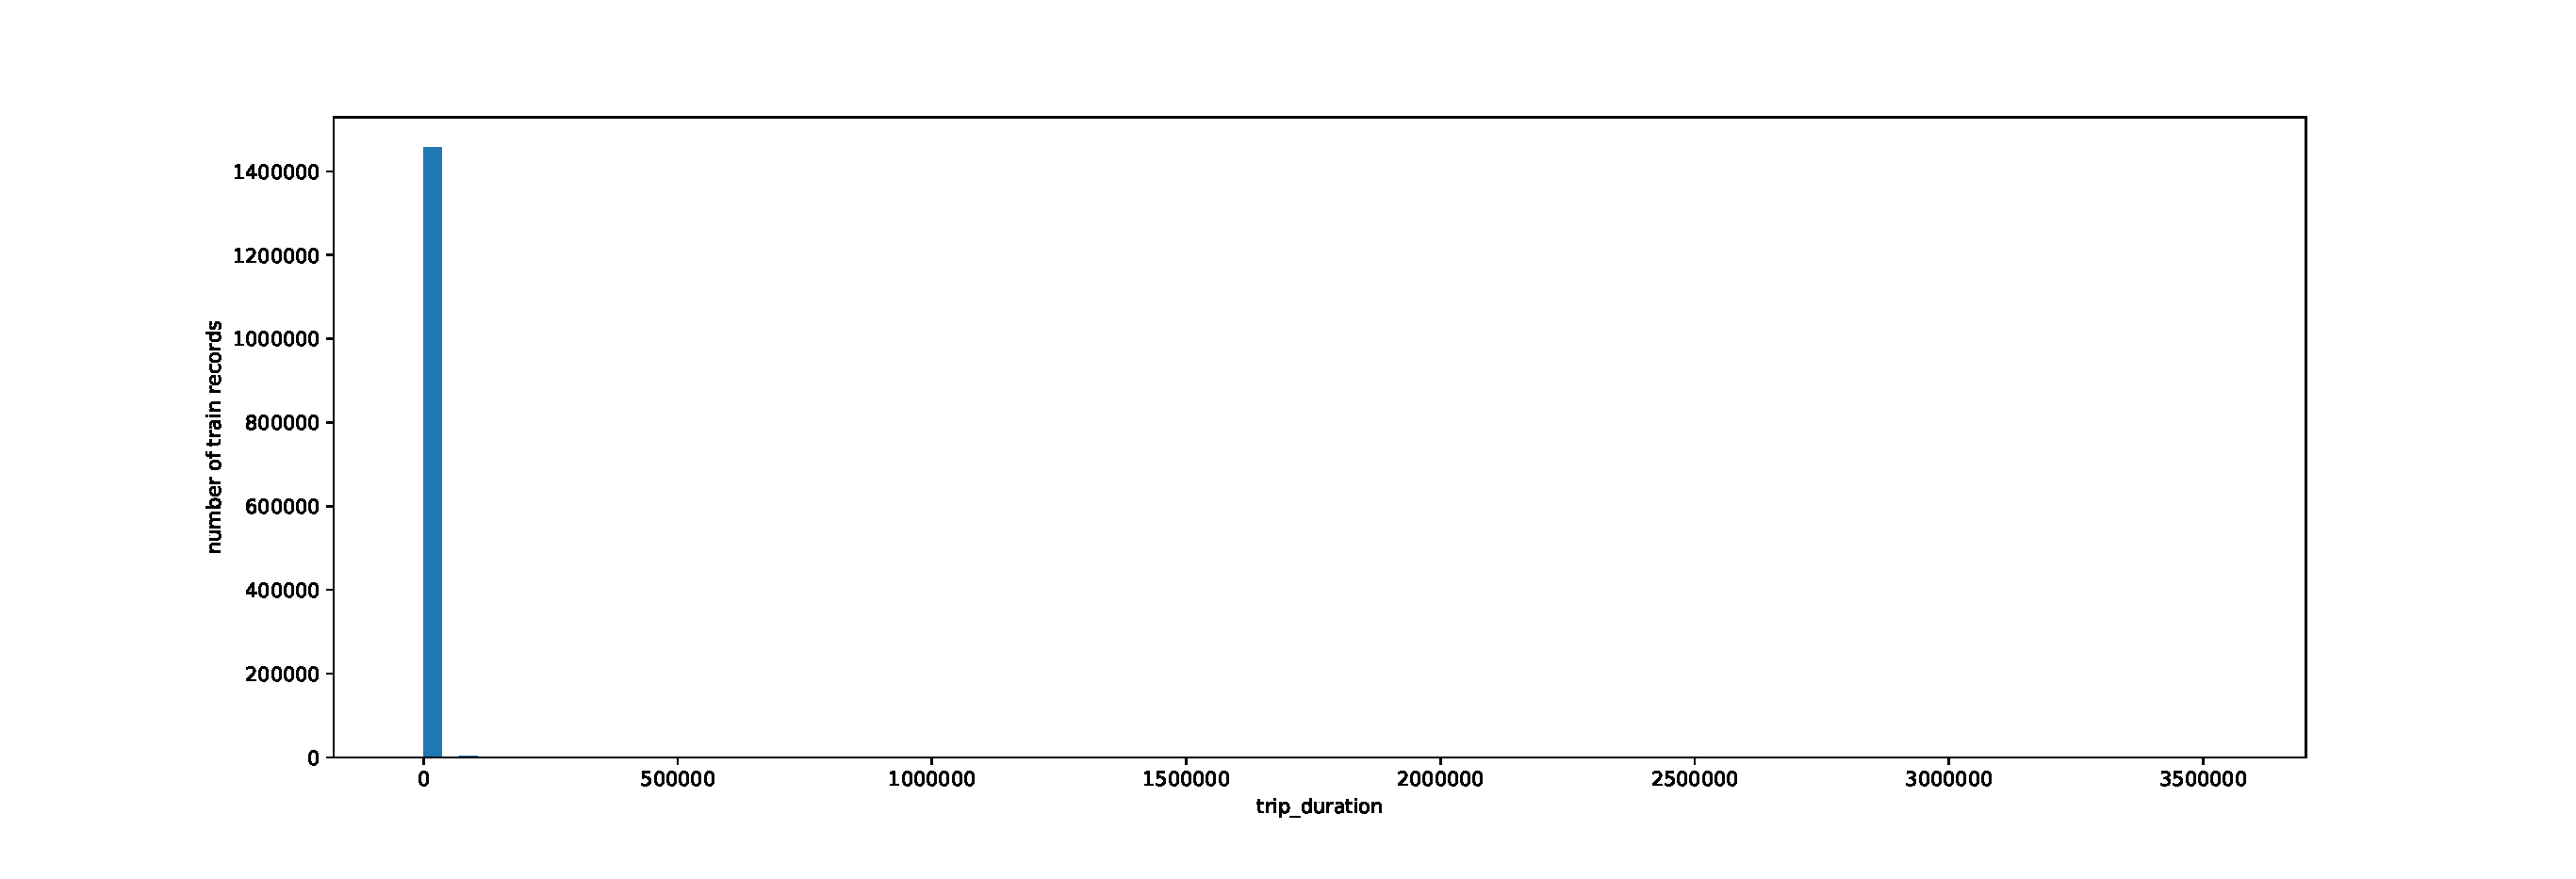
\includegraphics[width=0.8\textwidth]{figure//fig-1.eps}\\
  \caption{Visualize the distribution of trip-duration values}\label{fig:demical1}
\end{figure}



\section{Method} \label{sec-method}

%\blindtext

%\blindlist{itemize}[3] 
The method in this paper mainly focuses on data processing and feature analysis of the New York City Taxi Trip Duration, and then establishes multiple baseline models for comparison. The best prediction model is obtained according to the evaluation index.

\subsection{Outlier Processing}
The processing of outlier values should have different methods for each feature.
\begin{itemize}
    \item  
  According to the relationship between the position of longitude and latitude and the trip-duration, we can filter out the abnormal data. It can be clearly seen from Figure 1 that the travel time is mostly distributed within 1 million. Therefore, this article will delete the interference data that is not within 1 million. Selecting appropriate time data will help to train the model and improve the accuracy of the experiment.
   \item
  Passenger-count is the number of passengers in the vehicle. According to the analysis of Fig. 2, the number of passengers varies from 0 to 9. Therefore, we need to delete the data with 0 passengers.
  \end{itemize}

\begin{figure}
  \centering
  \selectcolormodel{rgb}
  %\missingfigure{Testing.}
   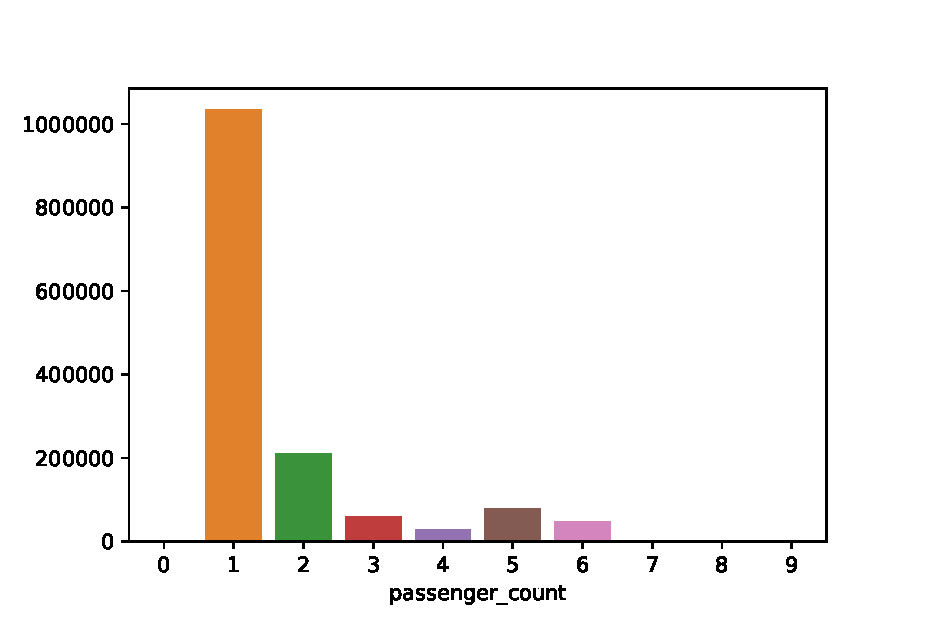
\includegraphics[width=0.8\textwidth]{figure//fig-2.eps}\\
  \caption{Visualize the distribution of passenger-count values}\label{fig:demical1}
\end{figure}

\begin{figure}
  \centering
  \selectcolormodel{rgb}
  %\missingfigure{Testing.}
   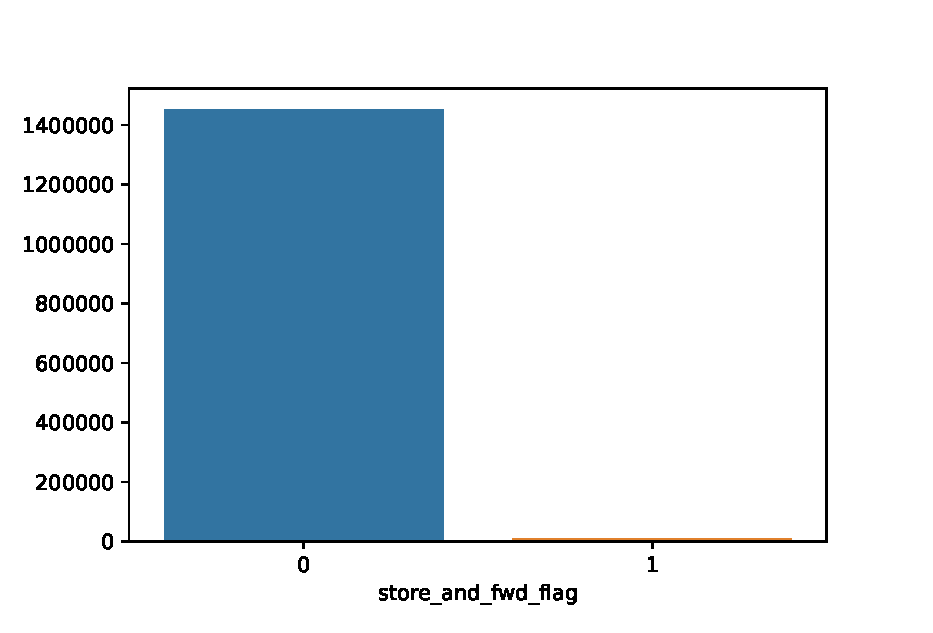
\includegraphics[width=0.6\textwidth]{figure//fig-4.eps}\\
  \caption{Visualize the distribution of store-and_fwd-flag}\label{fig:demical1}
\end{figure}

\subsection{Feature filtering}
Feature processing mainly deals with several special features of this paper.
\begin{itemize}
    \item  
   Store-and-fwd-flag indicates whether the trip record was held in vehicle memory before sending to the vendor because the vehicle did not have a connection to the server. Y=store and forward, N=not a store and forward trip. We convert its character identification into numbers for easy analysis. It can be clearly seen from Fig. 3 that the distribution of 0,1 is uneven.
    \item 
   Add month, week and day. From the perspective of the trend, the overall taxi time has been increasing from January to June 2016. It may be that users are gradually accustomed to taking a taxi from a longer distance, or it may be that more and more vehicles are driving on the road or the weather is bad, causing traffic congestion. In this article, the original pickup-datetime is divided into hour, day of week and month.
    \item 
   Create a distance feature. According to the longitude and latitude in the known data, the distance between the starting position and the ending position of the taxi is calculated according to the formula.
   \end{itemize}



\begin{figure}
  \centering
  \selectcolormodel{rgb}
  %\missingfigure{Testing.}
   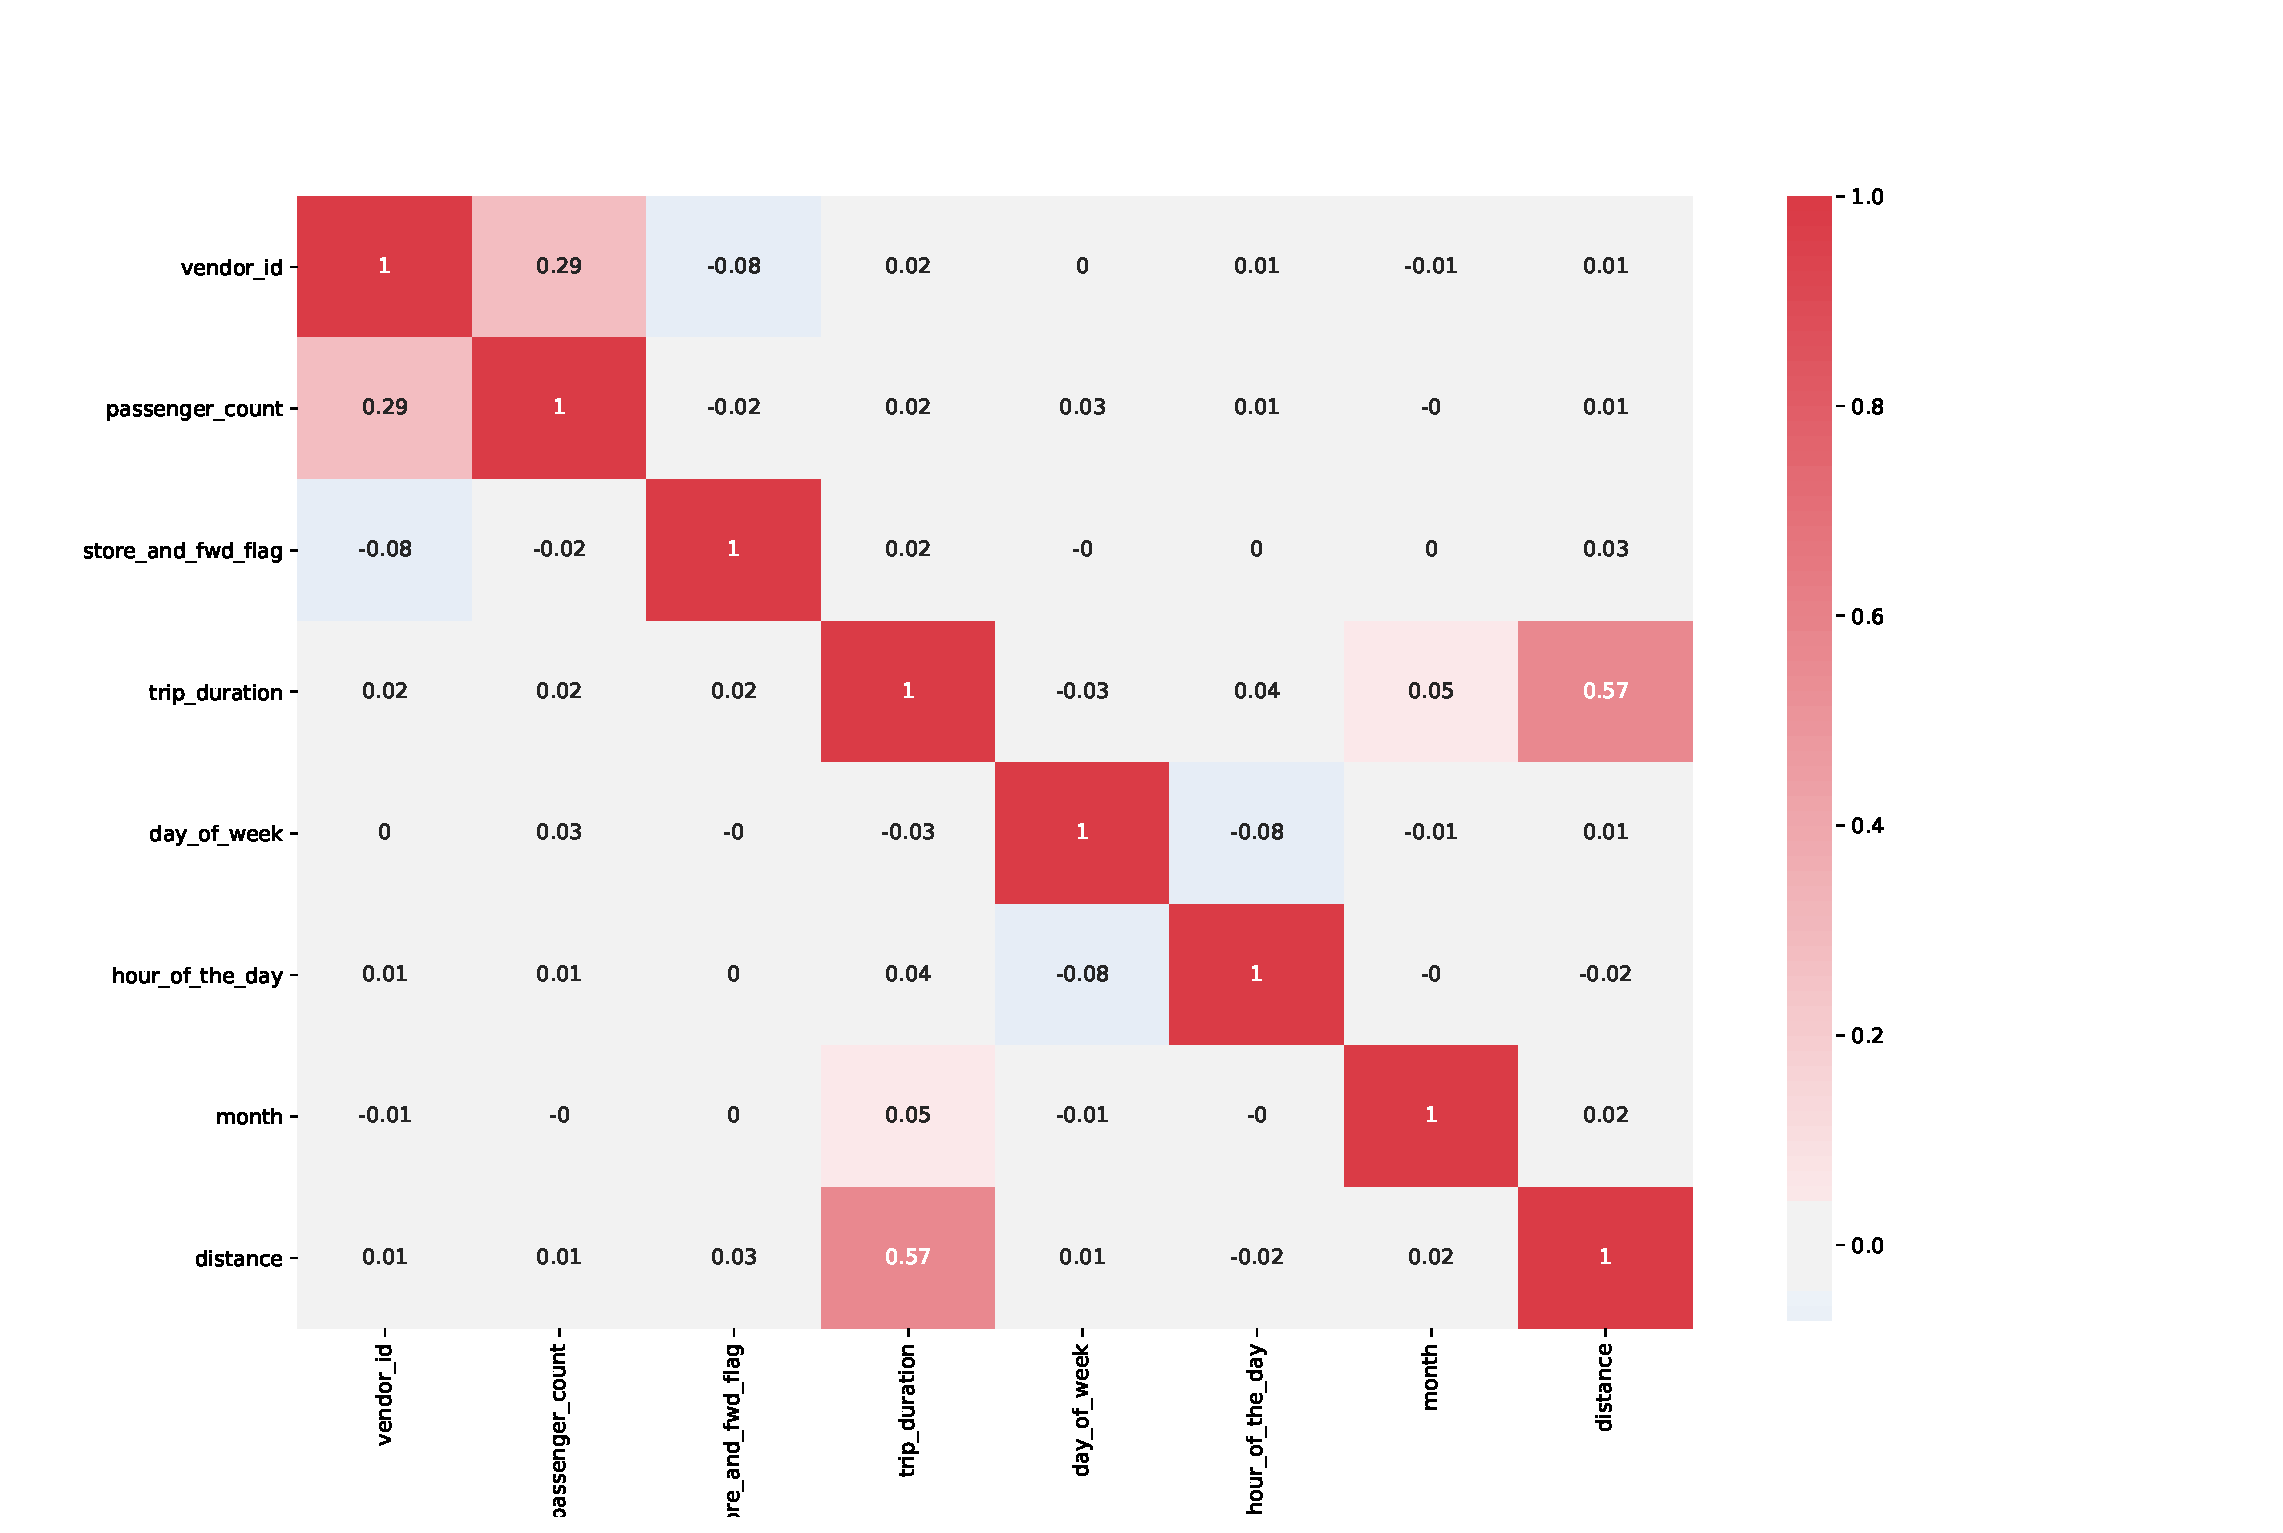
\includegraphics[width=0.7\textwidth]{figure//fig-6.eps}\\
  \caption{Features relationship heatmap}\label{fig:demical}
\end{figure}


%\blinditemize 
%\blindenumerate

%\blindmathtrue
%\blindmathfalse
%\blinddescription

%\qwuMarker %TODO: QWu Here





\section{Experiment and Analysis} \label{sec-experiment}
Three models were selected in this experiment: LGBMRegressor, LinearRegression and DecisionTreeRegressor. 
The division ratio of training set and test set is set to 0.3.


\subsection{Evaluation indicators}
In this paper, four evaluation indicators are used: R2-score, MAE, MSE, RMSE.

\begin{itemize}
    \item
${MSE = \frac{1}{m}{\sum\limits_{i = 1}^m {\left( {f\left( {{x_i}} \right) - {y_i}} \right)} ^2}}$

\item
${MAE = \frac{1}{N}\sum\limits_{i = 1}^N {\left| {{y_i} - f\left( {{x_i}} \right)} \right|} }$

\item
${RMSE = \sqrt {\frac{1}{N}\sum\limits_{i = 1}^N {{{\left( {{y_i} - f\left( {{x_i}} \right)} \right)}^2}} } }$

    
\end{itemize}


\begin{table}[]
\setlength{\abovecaptionskip}{0pt}
\setlength{\belowcaptionskip}{10pt}
\setlength{\tabcolsep}{10pt} % Default value: 6pt
\renewcommand{\arraystretch}{1.5} % Default value: 1
\centering
\caption{The experiment result on New York City Taxi Trip Duration}
\label{tbl:overall-experiments1}
\begin{tabular}{cccc}
\hline
\textbf{Model} & \textbf{LGBMRegressor}      & \textbf{LinearRegression} & \textbf{DecisionTreeRegressor} \\
\hline
R2\_score      & 0.66                        & 0.35                      & 0.3                            \\
MSE            & {\color[HTML]{FE0000} 0.22} & 0.42                      & 0.45                           \\
MAE            & {\color[HTML]{FE0000} 0.32} & 0.46                      & 0.46                           \\
RMSE           & {\color[HTML]{FE0000} 0.47} & 0.65                      & 0.67  \\
\hline
\end{tabular}
\end{table}

\subsection{Experimental analysis}
From~\cref{tbl:overall-experiments1}, it can be clearly seen from the experimental results that there are obvious differences in the evaluation effects of the three baseline models on the four evaluation indexes. Generally speaking, the evaluation value of LGBMRegressor model is better than other baseline models, and better evaluation results can be obtained.



\section{Conclusions} \label{sec-conclusions}
%\blindtext
The data of the simulation experiment of this project is from the real data of New York City Taxi Trip Duration, which is conducive to verifying the effectiveness of the model. In this project, the effects of 3 baseline models on 4 evaluation indexes are compared. Finally, it is found that the prediction effect of LGBMRegressor model is the best as a whole.

The analysis of this experiment can not only accurately predict the travel time of taxis, but also mine more detailed information about urban travel behavior. For example, it is possible to analyze which areas in which periods of time are more prone to orders, and where people generally go from which places - this is an effective data for rental scheduling. It can be inferred from the abnormal value brought by the blizzard that the weather is closely related to the order quantity. According to the weather data corresponding to the date, the impact of the weather and the order quantity can be further analyzed. Combined with the location data, it can also analyze which areas are greatly affected by the weather.

\section*{Acknowledgement}

\lipsum[1]


The authors would like to thank \ldots



% ----------------------------------------------------------------
\newpage
\bibliography{tuliplab,yourbib}
% TODO: you should change this yourbib into a proper bib file name
\bibliographystyle{plainnat}
%=================================================================

\listoftodos

\end{document}

